\section{Additional figures}
\label{sec:figs}
Figure~\ref{fig:overview} collects views referenced from the main paper: bearing
breadth, helped cells by stratum, retrieval, the representation contrasts with
their token costs, the cross-benchmark contrasts, and the two readers'
agreement. Figure~\ref{fig:lenctl} (Section~\ref{sec:lengthcontrol}) details the
length-control run.



\begin{figure*}[p]
\centering
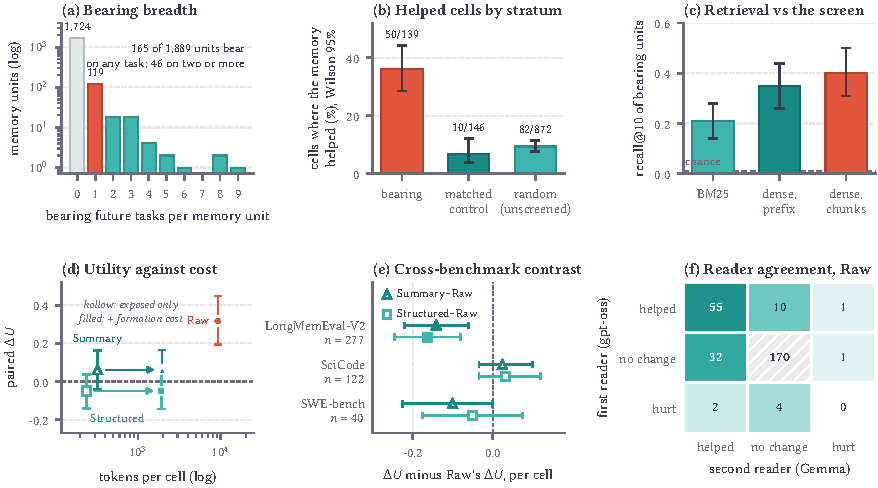
\includegraphics[width=\textwidth]{fig_results}
\caption{Overview of further results on LongMemEval-V2 (a--d, f) and across
benchmarks (e). \textbf{(a)}~Future tasks each of the $\bearUnits$ memory units
bears on, over $\bearDetTasks$ discriminative tasks (log axis).
\textbf{(b)}~Share of cells where the memory helped, cell-level Wilson 95\%
intervals (memory-resampled ones in Section~\ref{sec:negative}), for
the same $\spMems$ memories in three strata. \textbf{(c)}~Share of bearing units a retriever ranks in its top ten of the
domain pool (75 tasks, task-clustered 95\% intervals); the dashed line is
chance. \textbf{(d)}~Paired
\textsc{bearing}$-$control effect per representation ($\frCells$ cells,
$\frMems$ memories, intervals over memories); hollow markers count exposed
tokens, filled ones add formation cost amortized over $\frReuse$ cells.
\textbf{(e)}~Per-cell $\Delta U$ minus Raw's, task-clustered intervals; filled
markers exclude zero. \textbf{(f)}~Two readers' labels on $\rgSmCells$ Raw cells
in one session; the hatched cell (zero under both) cannot disagree.}
\label{fig:overview}
\Description{Six panels: a log histogram of bearing tasks per memory unit peaking at one; bar chart of helped-cell rates by stratum with bearing highest; similarity sextile lines nearly flat; utility against tokens showing Raw above zero and compressed representations near zero; cross-benchmark contrast intervals, only LongMemEval-V2 excluding zero; a three by three reader agreement table.}
\end{figure*}


